\documentclass{article}

%package setup
\usepackage{graphicx}
\usepackage{amsmath}
\usepackage{fancyhdr}
\usepackage[margin=1in]{geometry}
\usepackage{comment}
\usepackage{placeins}
\usepackage{parskip}
\usepackage{subcaption}
\usepackage{appendix}
\usepackage{soul}
\usepackage{comment}
\usepackage[hidelinks]{hyperref}
\usepackage{matlab-prettifier}
\usepackage{minted}
\usepackage{enumitem}
\usepackage{float}
\usepackage{textcomp, gensymb}

\pagestyle{fancy}
\fancyhf{} % Clear header/footer settings
\rhead{\thepage} % Page number on the right in the header
\lhead{ASE375 Lab Report 4} % Your lab report title on the left

\begin{document}

\begin{titlepage}
  \centering
  
\includegraphics[width=10cm]{ase-logo-formal.png}  % Adjust the width as needed
  \vspace{1cm}  % Add some vertical space
 
  \Large \textbf{ASE 375 Electromechanical Systems}\\
  \large \textbf{Section 14115}\\
  \vspace{0.5cm}
  \textbf{Monday: 3:00 - 6:00 pm}\\
 
  \vspace{1cm}
 
  \hrule
  \vspace{0.5cm}
 
  \Huge \textbf{Report 4:\\
  Measuring Pressure Vessels}\\
  \Huge \textbf{}\\
 
  \vspace{0.5cm}
  \hrule
 
  \vspace{1cm}
 
  \normalsize \textbf{Andrew Doty, Andres Suniaga, Dennis Hom}\\
  \normalsize \textbf{Due Date: 02/26/2024}
 
\end{titlepage}
\newpage

\tableofcontents
\thispagestyle{empty}
\newpage

\section{Introduction}
In this experiment we (1) Learn how to measure pressure with different sensors, (2) Construct a Wheatstone quarter-bridge circuit, and (3) Develop an understanding for strain gauge measurements. 

This is a two-part experiment of gathering output voltage readings from pressure changes of two vessels containing liquid. The first part involves calibrated pressure transducers and a full strain gauge bridge with a direct application of internal pressure to the vessel. The second part involves constructing a quarter-bridge circuit to read strain measurements on a soda can as pressure is released. These demonstrations set a foundation for understanding the precision and sensitivity of these sensors used to measure strain and pressure. 

\section{Equipment}
Devices and hardware used in this lab include:
\begin{itemize}

\item Digital Calipers: 
\vspace{1mm}

Used for measuring outer and inner dimensions of objects. In our case we use it to the measure the wall thickness of the soda can in $mm$.
\vspace{2.5mm}

\item PX309 SERIES Pressure Transducer/Transmitter:
\vspace{1mm}

Calibrated pressure transducer used to measure and convert pressure to an analog electrical signal or an output voltage. For this lab, the transducer is connected to a cylindrical poly-carbonate vessel containing liquid and is used alongside a full strain gauge bridge.
\vspace{2.5mm}

\item Strain Gauge: 
\vspace{1mm}

Sensor used to measure surface strains which then converts it into a change in electrical resistance. An output voltage is produced when a surface strain occurs since there is a resistance change within the bridge configuration. 
\vspace{2.5mm}

\item Cylindrical Poly-carbonate Vessel: 
\vspace{1mm}

A vessel containing a liquid equipped with a pressure transducer, full strain gauge bridge, a pressure regulator, and valves for the intake and release of pressure. We conduct Part 1 of gathering measurements with this vessel.
\vspace{2.5mm}

\item Aluminum Soda Can:
\vspace{1mm}

A full diet coke can strapped with a strain gauge sensor for Part 2 of measurements in this lab. The can is then opened to release the internal pressure for which we gather our strain measurement.
\vspace{2.5mm}

\item 320 Grit Sand Paper and Clear Tape: 
\vspace{1mm}

Used to smooth the surface of the Aluminum soda can. The strain gauge sensor can then be securely adhered to the surface of the soda can. The clear tape is for adhering the strain gauge to the surface of the soda can.

\item Pressure Regulator/Dial: 
\vspace{1mm}

A dial used to adjust the internal pressure of the Poly-carbonate vessel.
\vspace{2.5mm}

\item DAQ, NI-9215 Voltage Input Module, and LabVIEW:
\vspace{1mm}

Data Acquisition System used to process sample measurements into digital data. NI-9215 is an analog input module used to measure the output voltage signals of sensors and send it through the DAQ system. LabVIEW used to model these output voltages read from the DAQ of the transducer and strain gauge measurements.
\vspace{2.5mm}

\item Solderless Breadboard, Jumper Wires, and $350\Omega$ Resistors: 
\vspace{1mm}

Used to make connections to the input analog modules and to construct circuits. In Part 2 of this lab we build the Wheatstone quarter-bridge circuit with three $350\Omega$ resistors as shown below:

\begin{figure}[H]
    \centering
    \hypertarget{Fig1}{\frame{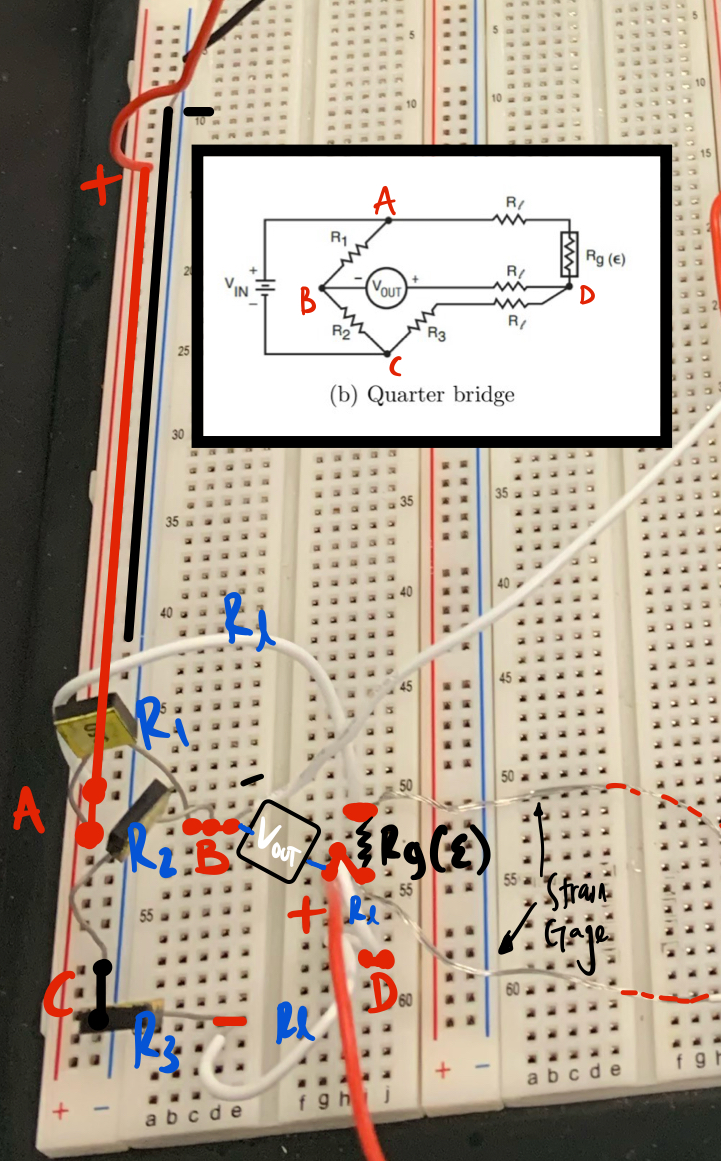
\includegraphics[width=0.65\textwidth]{lab4images/quarterbridge_circuit_lab4.jpg}}}
    \caption{Quarter-Bridge Configuration with the strain gauge resistance $R_{g}(\epsilon)$}
\end{figure}
\end{itemize}
\pagebreak

\section{Procedure}
The procedure for this experiment is broken up into two parts:
\subsection{Part 1: Poly-carbonate Vessel}
\begin{figure}[H]
    \centering
    \frame{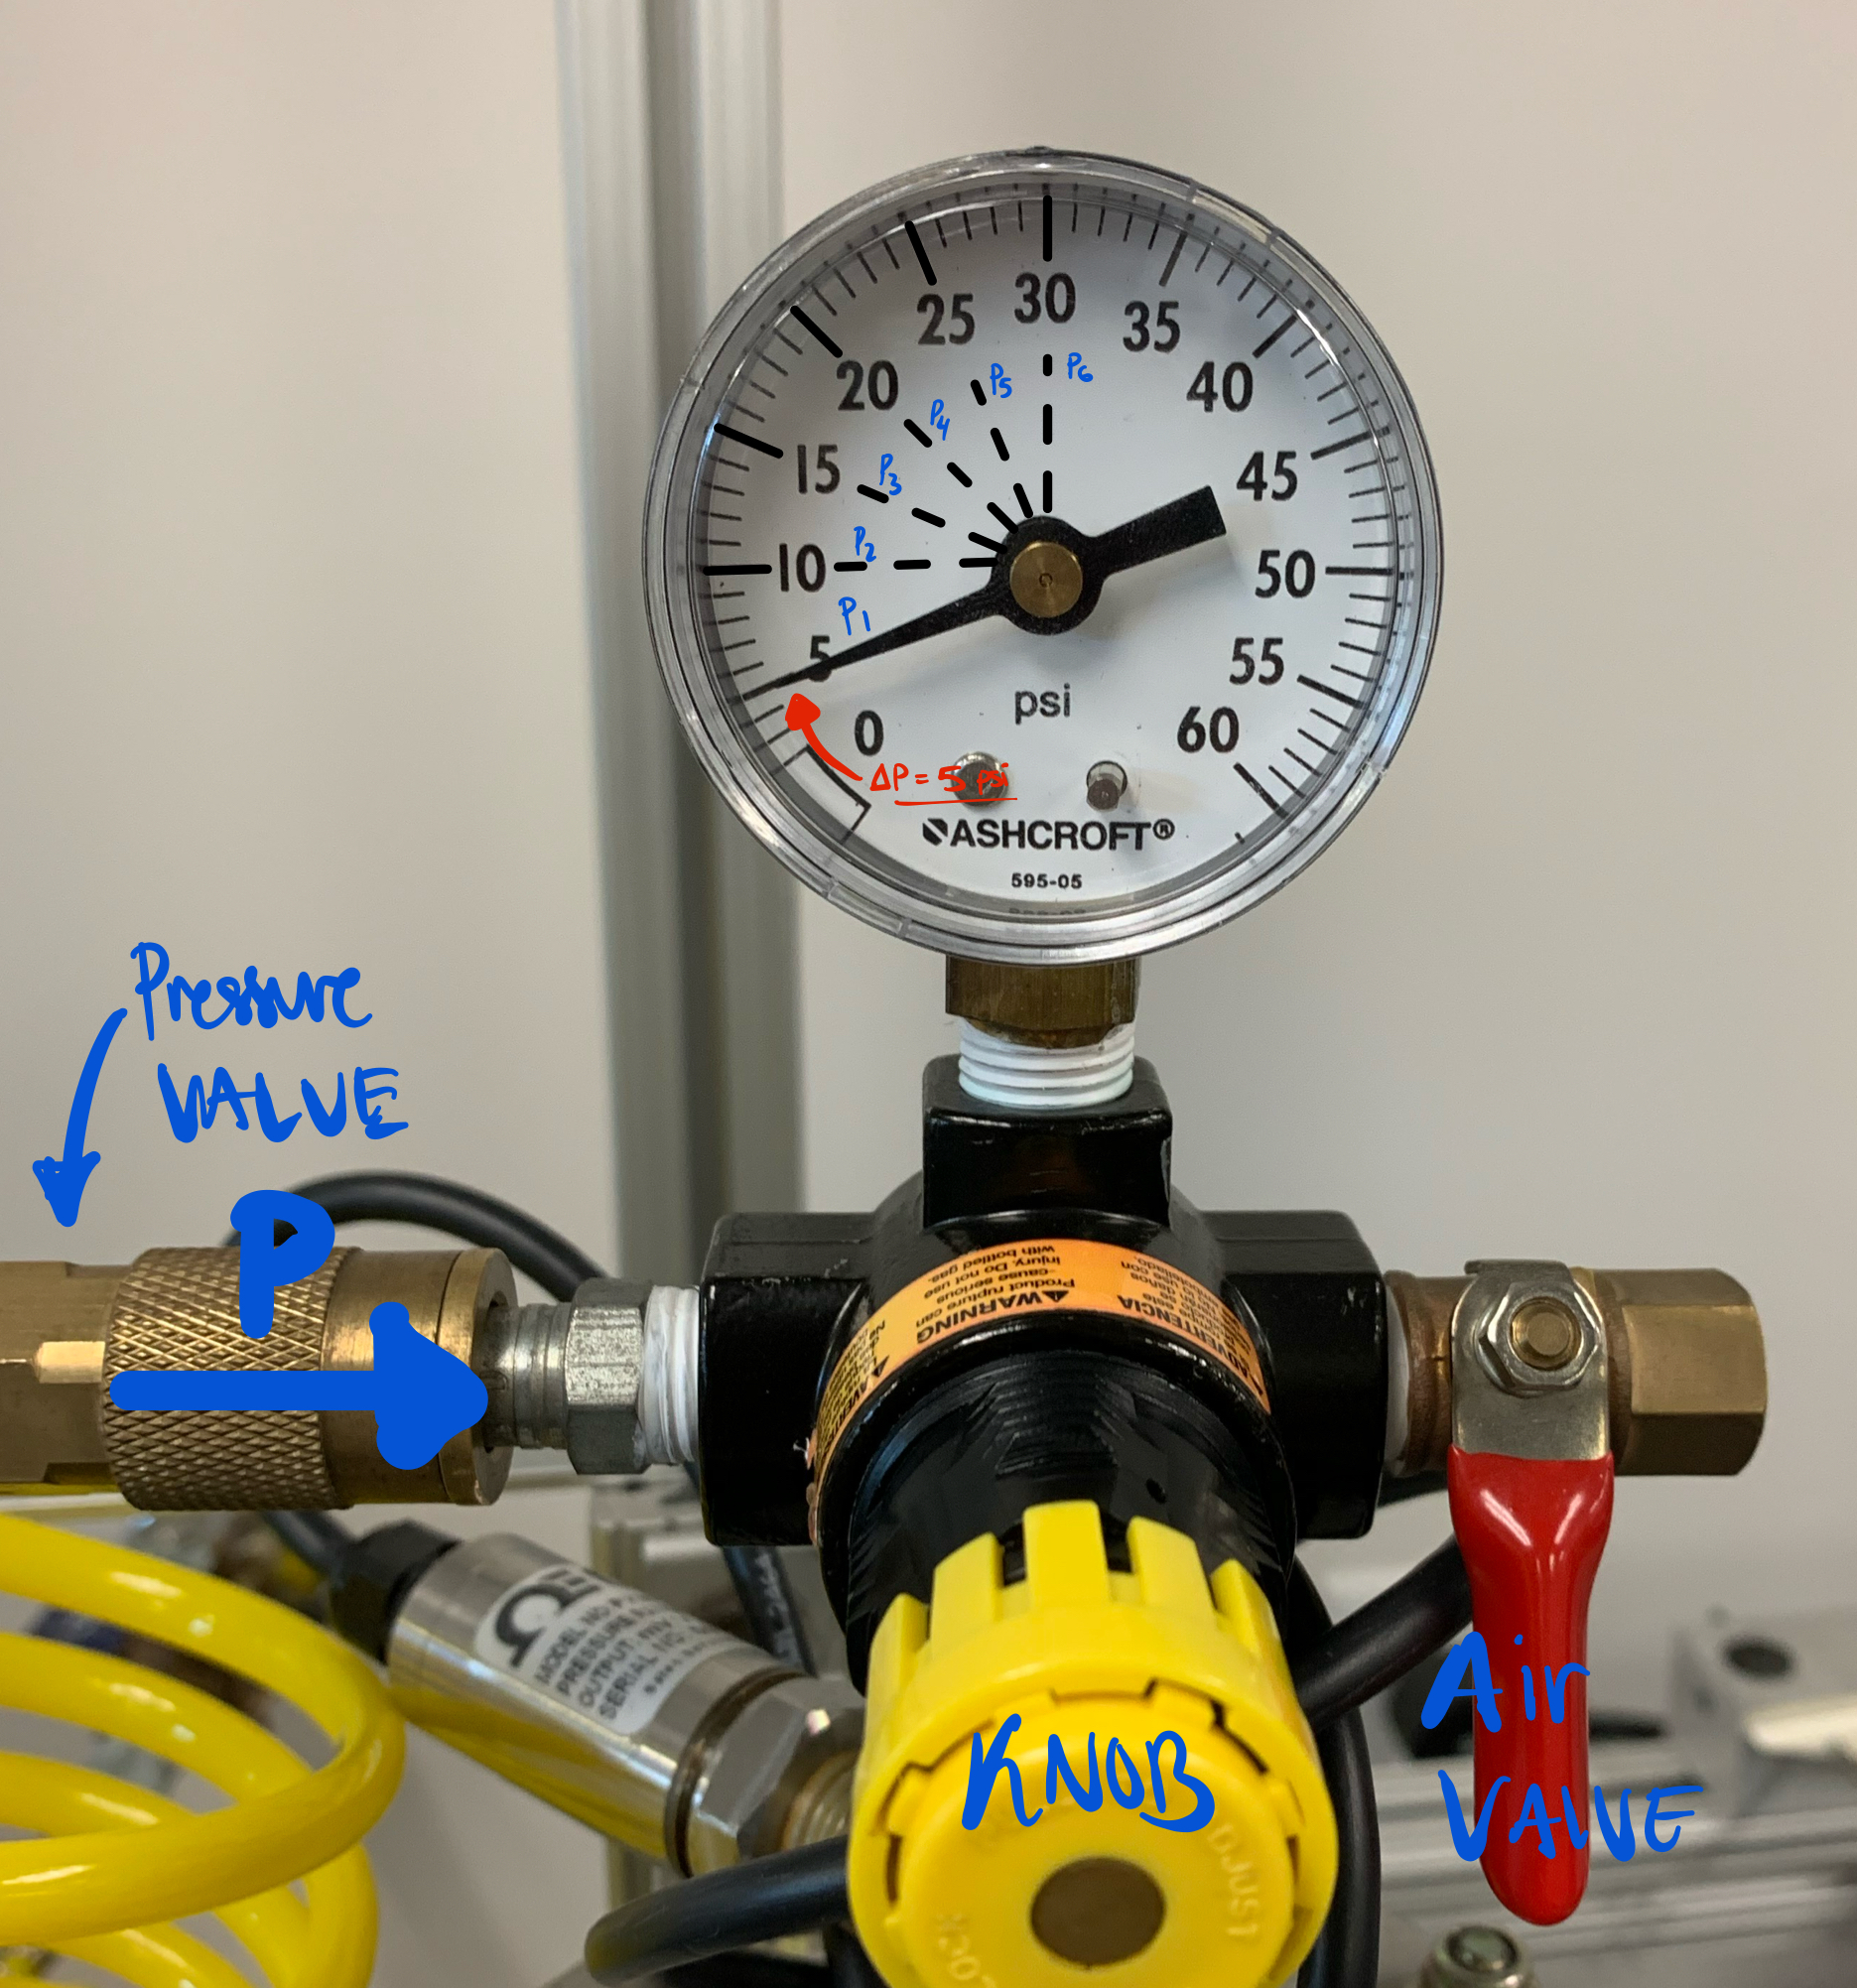
\includegraphics[width=0.5\textwidth]{lab4images/pressuregage_lab4.jpg}}
    \caption{Part 1: Devices Attached to the Poly-carbonate Vessel}
\end{figure}

\begin{enumerate}
    \item Make sure all connections from the pressure transducer and Wheatstone bridge are powered and connected to the input analog module (NI-9215). Set up and run LabVIEW to plot the output voltages.
    \item Before starting to adjust the pressure dial, \underline{release all the pressure or air from the vessel}. To do this, close the pressure valve and twist the air valve slightly such that it was open about a quarter of the way (labeled in \textbf{Figure (2)}). Unlock the knob and carefully increase the pressure dial until you hear the release of air. Let it release slowly. Once all the air has been released, turn back the knob and lock it, close the air valve, and open the pressure valve. 
    \item Start by marking down the $P_{0} = 0\, psi$ pressure readings of the pressure transducer and Wheatstone bridge sensors from LabVIEW. 
    \item Unlock the knob and slowly twist it until the pressure dial hand turns $\Delta P$ to the next pressure $P_{1}$. Lock in the knob. We choose $P_{1} = 5\, psi$ using step $\Delta P = 5\, psi$ for our measurements. 
    \item Ensure the plot of the output voltage approaches an approximate steady state. Record the data of each sensor for $P_{1}$ and unlock and move the dial again by $\Delta P$ to $P_{2}$. Lock the knob and record the output voltages at $P_{2}$. 
    \item Repeat $\Delta P$ movements of the pressure dial up to $P_{f}$ (at least 5 or 6 measurements), not to exceed $P_{max} = 50\, psi$. Record the output voltage of each sensor from LabVIEW for each $P_{i}$. We chose to gather $i=6$ measurements so that $P_{f} = P_{6} = 30\, psi$.
    \item Once finished, close the pressure valve and turn the knob all the way back to $0$. Slightly and slowly open the air valve again to release all the pressure. This may require carefully increasing the knob to release the rest of the air. After all the air is out, close the air valve and turn the knob all the way back and lock it. 
    \item With these output voltage readings we can now process this data to obtain a pressure measurement from the sensors.
    \end{enumerate}

\subsection{Part 2: Aluminum Soda Can}
\begin{enumerate}
    \item Acquire the soda can and begin sanding a spot on the surface of the soda can until the spot is just the plain aluminum surface (or sand for $\approx 1$ min). This is to smoothen out the surface of the soda can in order to make adhesion easier.
    \item With the clear tape, stick the strain gauge on the plain aluminum surface of the soda can.
    \item Grab three $350\Omega$ resistors and jumper wires. Construct the quarter-bridge circuit as seen in \hyperlink{Fig1}{\textbf{Figure (1)}} with the Strain Gauge. For measuring the output voltage $V_{OUT}$, connect wires from the null center of the bridge to the NI-9215.
    \item Run LabVIEW to test the sensor. Place a finger on the strain gauge and carefully apply force to check that the resulting $V_{OUT}$ changes on the plot in LabVIEW. The null center voltage will no longer be $0$ (or null). In fact it will decrease (constant current) as the gauge resistance increases with increasing strain.
    \item After testing the strain gauge, record the change in output voltage as the soda can is opened (releasing pressure within the can). Ensure this data is written to a spreadsheet for data processing.
    \item With the collection of output voltages we can model the change in pressure and determine the pressure inside the unopened can. Next up: \textbf{Data Processing}.
\end{enumerate}

\section{Data Processing}
\subsection{Variables and Equations}
\begin{enumerate}[label = \Roman*.]
    \item 
\end{enumerate}

For part 1, our first values will be in voltages. We will convert these to pressures using the following equation:
\[
P = \frac{V}{0.004} - 14.7
\]

What are any of the sources of error or discrepancies in the data? How can we account for these?
- The gauge on the pressure vessel may not be accurate
- The true measurements were likely taken with an inaccurate gauge, and our uncertainties are likely larger than we think
- Over time, the pressure vessel leaked
- The pressure vessel could be at a different temperature than the room temperature
- The DAQ could be interpreting the data incorrectly from an error in the voltage.
- Delay in pressure changes from the valve opening.


\section{Results and Analysis}

\section{Conclusion}

\newpage
\thispagestyle{empty}  % Clear header/footer
\begin{center}
	\vspace*{\fill}
	{\Huge Appendices}
	\vspace*{\fill}
\end{center}

% Start appendices
\newpage
\begin{appendices}
\pagestyle{fancy}
\renewcommand{\thefigure}{A\arabic{figure}}
\setcounter{figure}{0}

\section*{Appendix: t-Distribution Tables}
\hypertarget{1}{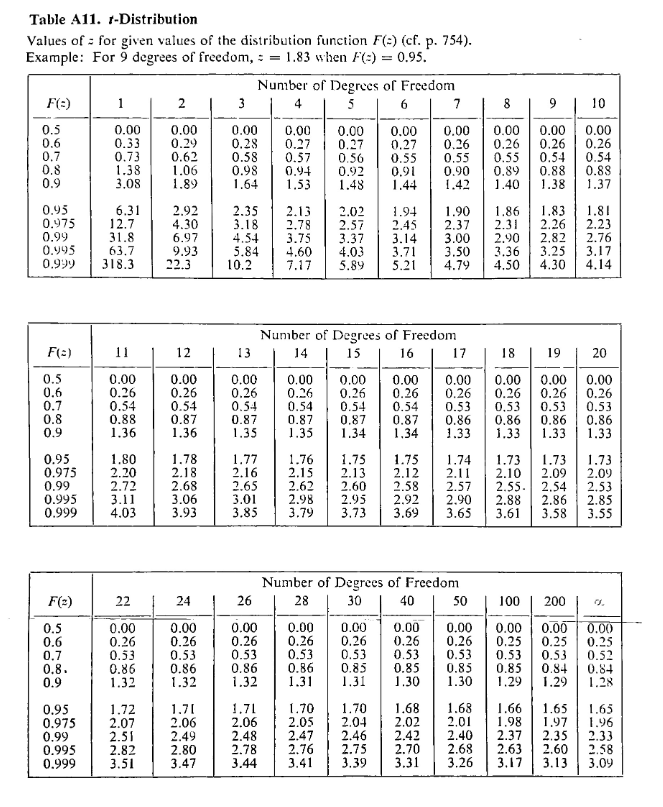
\includegraphics[width=0.95\textwidth]{t_distribution_Table_lecture3.png}}

\section*{Appendix: NI-9215 Datasheet}
\href{https://www.amc-systeme.de/files/pdf/ni-9215-amc.pdf}{NI-9215 Datasheet}
\end{appendices}

\end{document}
